\subsection{Results for Heading}
%\label{subsec:direction_results}
%\vspace{10pt}

Figure~\ref{fig:var_direction} represents the $p$-values for the Wilcoxon signed-rank test on actual and predicted values across $k$-fold validation datasets for the heading in the $k$-fold testing datasets using different RNN models, and forecasting times. Darker colors in grayscale represent a higher $p$-value in a range from $0$ to $1$. The values on the secondary diagonal are all equal to $1$ and black because models equal themselves.

\begin{figure}[!ht]
	\centering
	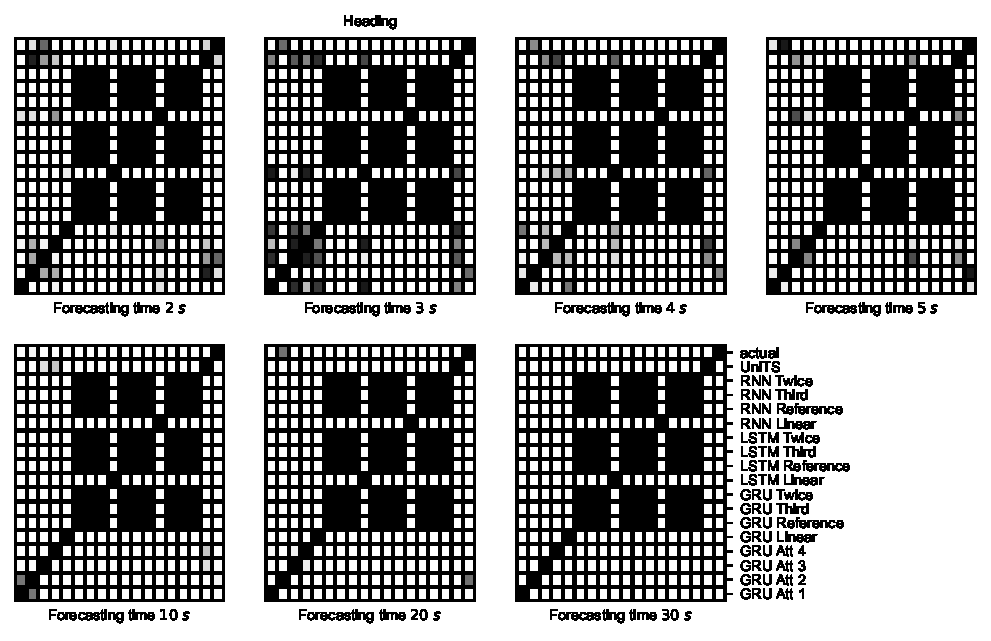
\includegraphics[width = 0.99 \linewidth]{var_direction.pdf}
	\caption{The $p$-values for the Wilcoxon signed-rank test on actual and predicted values across $k$-fold validation datasets for the heading in the $k$-fold testing datasets using different RNN models, and forecasting times. Darker colors in grayscale represent a higher $p$-value in a range from $0$ to $1$. The values on the secondary diagonal are all equal to $1$ and black because models equal themselves.}
	\label{fig:var_direction}
\end{figure}

Figure~\ref{fig:best_RMSE_val} contains the average RMSE across $k$-fold testing datasets using different validation datasets for all variables estimated in nested $k$-fold cross-validation by different RNN models, and forecasting times.

\begin{figure}[!ht]
	\centering
	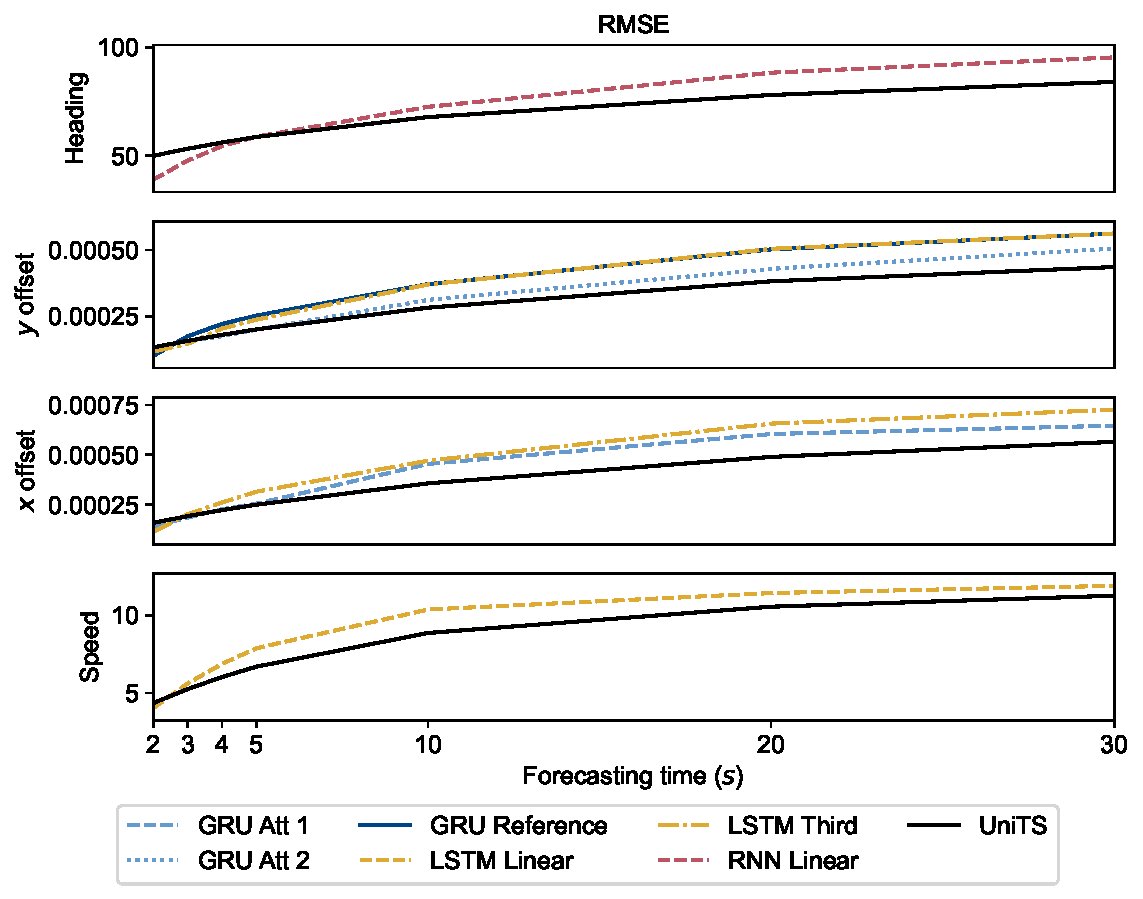
\includegraphics[width = 0.99 \linewidth]{best_RMSE_val.pdf}
	\caption{The average RMSE across $k$-fold testing datasets using different validation datasets for all variables estimated in nested $k$-fold cross-validation by different RNN models, and forecasting times.}
	\label{fig:best_RMSE_val}
\end{figure}

The average RMSE, with standard deviation in brackets, across $k$-fold validation datasets for the heading estimated on the $k$-fold testing datasets by different RNN models, and forecasting times is listed in Table~\ref{tab:best_direction_RMSE}.

\begin{table}[!ht]
	\centering
	\resizebox{\linewidth}{!}{
		\begin{tabular}{|c|c|c|c|c|c|c|c|}
			\hline
			Model & $2$ $s$ & $3$ $s$ & $4$ $s$ & $5$ $s$ & $10$ $s$ & $20$ $s$ & $30$ $s$ \\ \hline
			\multirow{2}{*}{RNN Linear} & $\mathbf{38.85}$ & $\mathbf{47.63}$ & $\mathbf{54.36}$ & $58.71$ & $72.54$ & $88.35$ & $95.47$ \\
			 & \textbf{(}$\mathbf{1.85}$\textbf{)} & \textbf{(}$\mathbf{2.42}$\textbf{)} & \textbf{(}$\mathbf{2.22}$\textbf{)} & ($2.05$) & ($2.33$) & ($1.93$) & ($2.48$) \\ \hline
			\multirow{2}{*}{UniTS} & $49.88$ & $53.14$ & $56.02$ & $\mathbf{58.6}$ & $\mathbf{67.8}$ & $\mathbf{78.04}$ & $\mathbf{84.09}$ \\
			 & ($2.18$) & ($2.29$) & ($2.35$) & \textbf{(}$\mathbf{2.38}$\textbf{)} & \textbf{(}$\mathbf{2.26}$\textbf{)} & \textbf{(}$\mathbf{2.29}$\textbf{)} & \textbf{(}$\mathbf{2.47}$\textbf{)} \\ \hline
		\end{tabular}
	}
	\caption{The average RMSE, with standard deviation in brackets, across $k$-fold validation datasets for the heading estimated on the $k$-fold testing datasets by different RNN models, and forecasting times.}
	\label{tab:best_direction_RMSE}
\end{table}

The RNN Linear model achieved the lowest RMSE for heading, and a forecasting time of $2$, $3$, and $4$ $s$ with average values and standard deviation (in brackets) that equal $38.85$ $\degree$ ($1.85$ $\degree$), $47.63$ $\degree$ ($2.42$ $\degree$), and $54.36$ $\degree$ ($2.22$ $\degree$) respectively.

The RNN Linear model does not have a statistically significantly different RMSE than the GRU Linear model for heading using a forecasting time of $2$ $s$, with a $p$-value equaling $3.764 \times 10^{-4}$.

The RNN Linear model does not have a statistically significantly different RMSE than the GRU Linear, and LSTM Linear models for heading using a forecasting time of $4$ $s$, with $p$-values equaling $5.564 \times 10^{-4}$, and $4.895 \times 10^{-4}$.

The UniTS model achieved the lowest RMSE for heading, and a forecasting time of $5$, $10$, $20$, and $30$ $s$ with average values and standard deviation (in brackets) that equal $58.6$ $\degree$ ($2.38$ $\degree$), $67.8$ $\degree$ ($2.26$ $\degree$), $78.04$ $\degree$ ($2.29$ $\degree$), and $84.09$ $\degree$ ($2.47$ $\degree$) respectively.

The UniTS model does not have a statistically significantly different RMSE than the LSTM Linear, and RNN Linear models for heading using a forecasting time of $5$ $s$, with $p$-values equaling $2.785 \times 10^{-3}$, and $6.721 \times 10^{-1}$.

\subsection{Results for $y$ Offset}
%\label{subsec:latitude_no_abs_results}
%\vspace{10pt}

Figure~\ref{fig:var_lat} represents the $p$-values for the Wilcoxon signed-rank test on actual and predicted values across $k$-fold validation datasets for the $y$ offset in the $k$-fold testing datasets using different RNN models, and forecasting times. Darker colors in grayscale represent a higher $p$-value in a range from $0$ to $1$. The values on the secondary diagonal are all equal to $1$ and black because models equal themselves.

\begin{figure}[!ht]
	\centering
	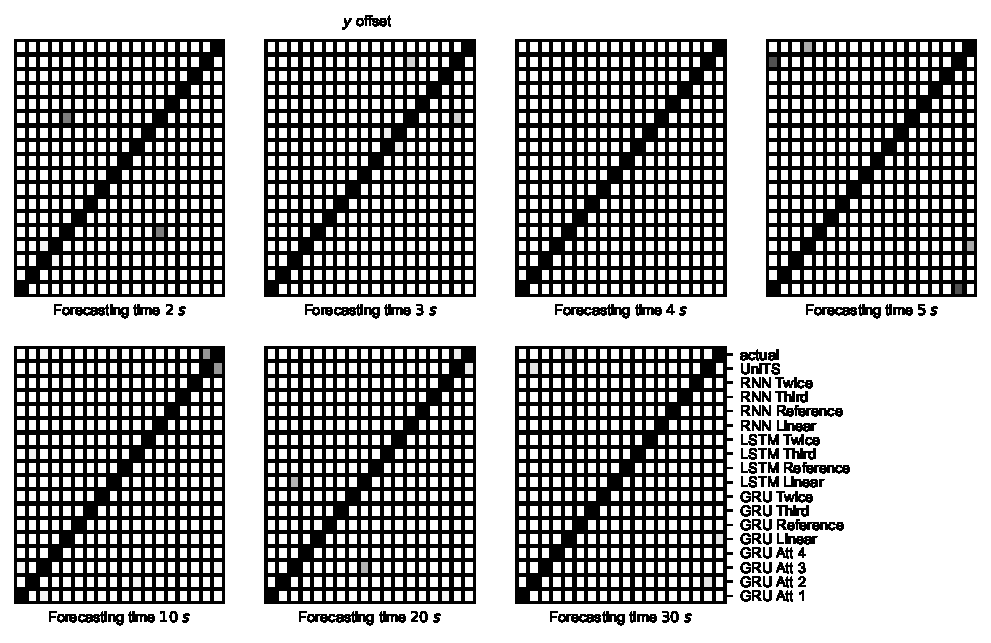
\includegraphics[width = 0.99 \linewidth]{var_lat.pdf}
	\caption{The $p$-values for the Wilcoxon signed-rank test on actual and predicted values across $k$-fold validation datasets for the $y$ offset in the $k$-fold testing datasets using different RNN models, and forecasting times. Darker colors in grayscale represent a higher $p$-value in a range from $0$ to $1$. The values on the secondary diagonal are all equal to $1$ and black because models equal themselves.}
	\label{fig:var_lat}
\end{figure}

The average RMSE ($\times 10^{-4}$), with standard deviation in brackets, across $k$-fold validation datasets for the $y$ offset estimated on the $k$-fold testing datasets by different RNN models, and forecasting times is listed in Table~\ref{tab:best_latitude_no_abs_RMSE}.

\begin{table}[!ht]
	\centering
	\resizebox{\linewidth}{!}{
		\begin{tabular}{|c|c|c|c|c|c|c|c|}
			\hline
			Model & $2$ $s$ & $3$ $s$ & $4$ $s$ & $5$ $s$ & $10$ $s$ & $20$ $s$ & $30$ $s$ \\ \hline
			\multirow{2}{*}{GRU Att 2} & $1.302$ & $1.584$ & $\mathbf{1.76}$ & $\mathbf{2.007}$ & $3.125$ & $4.289$ & $5.054$ \\
			 & ($0.207$) & ($0.238$) & \textbf{(}$\mathbf{0.198}$\textbf{)} & \textbf{(}$\mathbf{0.213}$\textbf{)} & ($0.26$) & ($0.325$) & ($0.438$) \\ \hline
			\multirow{2}{*}{GRU Reference} & $\mathbf{1.027}$ & $1.757$ & $2.219$ & $2.533$ & $3.711$ & $5.019$ & $5.615$ \\
			 & \textbf{(}$\mathbf{0.266}$\textbf{)} & ($0.357$) & ($0.352$) & ($0.251$) & ($0.276$) & ($0.34$) & ($0.395$) \\ \hline
			\multirow{2}{*}{LSTM Third} & $1.189$ & $\mathbf{1.473}$ & $2.049$ & $2.383$ & $3.701$ & $5.04$ & $5.616$ \\
			 & ($0.346$) & \textbf{(}$\mathbf{0.36}$\textbf{)} & ($0.479$) & ($0.349$) & ($0.23$) & ($0.386$) & ($0.406$) \\ \hline
			\multirow{2}{*}{UniTS} & $1.343$ & $1.586$ & $1.811$ & $2.017$ & $\mathbf{2.831}$ & $\mathbf{3.821}$ & $\mathbf{4.357}$ \\
			 & ($0.248$) & ($0.217$) & ($0.21$) & ($0.21$) & \textbf{(}$\mathbf{0.238}$\textbf{)} & \textbf{(}$\mathbf{0.301}$\textbf{)} & \textbf{(}$\mathbf{0.331}$\textbf{)} \\ \hline
		\end{tabular}
	}
	\caption{The average RMSE ($\times 10^{-4}$), with standard deviation in brackets, across $k$-fold validation datasets for the $y$ offset estimated on the $k$-fold testing datasets by different RNN models, and forecasting times.}
	\label{tab:best_latitude_no_abs_RMSE}
\end{table}

The GRU Att 2 model achieved the lowest RMSE for $y$ offset, and a forecasting time of $4$, and $5$ $s$ with average values and standard deviation (in brackets) that equal $17.603 \times 10^{-5}$ $\degree$ ($1.979 \times 10^{-5}$ $\degree$), and $20.067 \times 10^{-5}$ $\degree$ ($2.131 \times 10^{-5}$ $\degree$) respectively.

The GRU Att 2 model does not have a statistically significantly different RMSE than the GRU Att 1, LSTM Third, LSTM Twice, and UniTS models for $y$ offset using a forecasting time of $4$ $s$, with $p$-values equaling $2.551 \times 10^{-2}$, $4.605 \times 10^{-3}$, $1.453 \times 10^{-3}$, and $6.129 \times 10^{-3}$.

The GRU Att 2 model does not have a statistically significantly different RMSE than the GRU Att 1, and UniTS models for $y$ offset using a forecasting time of $5$ $s$, with $p$-values equaling $1.355 \times 10^{-2}$, and $3.525 \times 10^{-1}$.

The GRU Reference model achieved the lowest RMSE for $y$ offset, and a forecasting time of $2$ $s$ with an average value and standard deviation (in brackets) that equals $10.265 \times 10^{-5}$ $\degree$ ($2.66 \times 10^{-5}$ $\degree$).

The GRU Reference model does not have a statistically significantly different RMSE than the GRU Att 1, GRU Linear, GRU Third, GRU Twice, LSTM Linear, LSTM Reference, and LSTM Third models for $y$ offset using a forecasting time of $2$ $s$, with $p$-values equaling $3.781 \times 10^{-3}$, $1.908 \times 10^{-1}$, $9.573 \times 10^{-2}$, $6.338 \times 10^{-1}$, $3.419 \times 10^{-3}$, $1.485 \times 10^{-1}$, and $9.032 \times 10^{-2}$.

The LSTM Third model achieved the lowest RMSE for $y$ offset, and a forecasting time of $3$ $s$ with an average value and standard deviation (in brackets) that equals $14.733 \times 10^{-5}$ $\degree$ ($3.604 \times 10^{-5}$ $\degree$).

The LSTM Third model does not have a statistically significantly different RMSE than the GRU Att 1, GRU Att 2, GRU Att 3, GRU Att 4, GRU Linear, GRU Reference, GRU Third, GRU Twice, LSTM Linear, LSTM Reference, and UniTS models for $y$ offset using a forecasting time of $3$ $s$, with $p$-values equaling $1.874 \times 10^{-2}$, $2.748 \times 10^{-2}$, $4.895 \times 10^{-4}$, $3.088 \times 10^{-3}$, $5.072 \times 10^{-3}$, $1.027 \times 10^{-3}$, $9.032 \times 10^{-2}$, $6.721 \times 10^{-1}$, $2.191 \times 10^{-2}$, $4.605 \times 10^{-3}$, and $8.822 \times 10^{-3}$.

The UniTS model achieved the lowest RMSE for $y$ offset, and a forecasting time of $10$, $20$, and $30$ $s$ with average values and standard deviation (in brackets) that equal $28.309 \times 10^{-5}$ $\degree$ ($2.382 \times 10^{-5}$ $\degree$), $38.21 \times 10^{-5}$ $\degree$ ($3.005 \times 10^{-5}$ $\degree$), and $43.569 \times 10^{-5}$ $\degree$ ($3.311 \times 10^{-5}$ $\degree$) respectively.

\subsection{Results for $x$ Offset}
%\label{subsec:longitude_no_abs_results}
%\vspace{10pt}

Figure~\ref{fig:var_long} represents the $p$-values for the Wilcoxon signed-rank test on actual and predicted values across $k$-fold validation datasets for the $x$ offset in the $k$-fold testing datasets using different RNN models, and forecasting times. Darker colors in grayscale represent a higher $p$-value in a range from $0$ to $1$. The values on the secondary diagonal are all equal to $1$ and black because models equal themselves.

\begin{figure}[!ht]
	\centering
	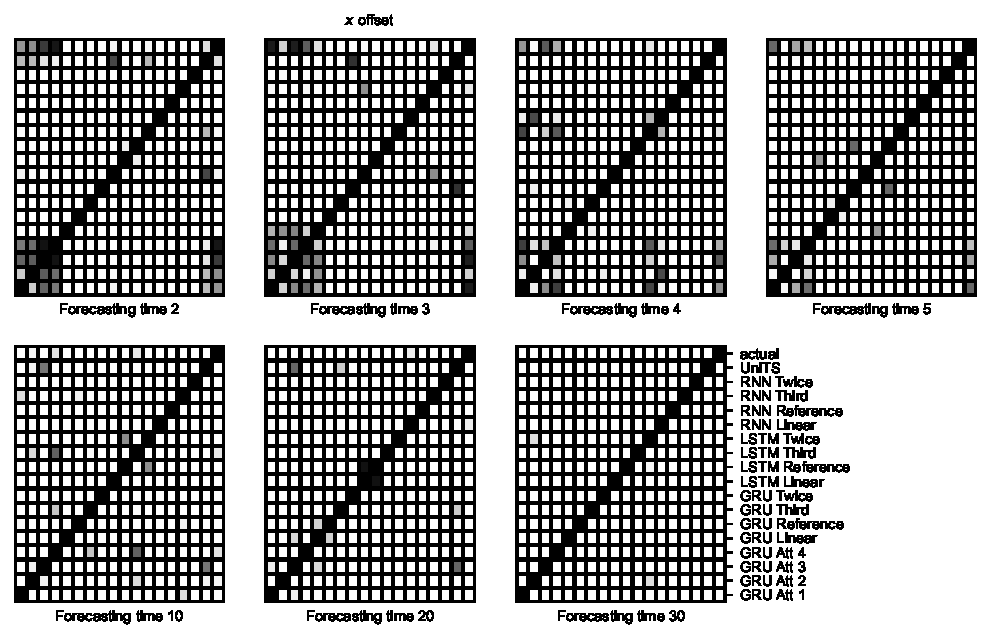
\includegraphics[width = 0.99 \linewidth]{var_long.pdf}
	\caption{The $p$-values for the Wilcoxon signed-rank test on actual and predicted values across $k$-fold validation datasets for the $x$ offset in the $k$-fold testing datasets using different RNN models, and forecasting times. Darker colors in grayscale represent a higher $p$-value in a range from $0$ to $1$. The values on the secondary diagonal are all equal to $1$ and black because models equal themselves.}
	\label{fig:var_long}
\end{figure}

The average RMSE ($\times 10^{-4}$), with standard deviation in brackets, across $k$-fold validation datasets for the $x$ offset estimated on the $k$-fold testing datasets by different RNN models, and forecasting times is listed in Table~\ref{tab:best_longitude_no_abs_RMSE}.

\begin{table}[!ht]
	\centering
	\resizebox{\linewidth}{!}{
		\begin{tabular}{|c|c|c|c|c|c|c|c|}
			\hline
			Model & $2$ $s$ & $3$ $s$ & $4$ $s$ & $5$ $s$ & $10$ $s$ & $20$ $s$ & $30$ $s$ \\ \hline
			\multirow{2}{*}{GRU Att 1} & $1.4$ & $\mathbf{1.85}$ & $2.26$ & $2.54$ & $4.54$ & $6.05$ & $6.47$ \\
			 & ($0.19$) & \textbf{(}$\mathbf{0.24}$\textbf{)} & ($0.27$) & ($0.27$) & ($0.69$) & ($0.47$) & ($0.6$) \\ \hline
			\multirow{2}{*}{LSTM Third} & $\mathbf{1.12}$ & $2.01$ & $2.6$ & $3.14$ & $4.7$ & $6.57$ & $7.27$ \\
			 & \textbf{(}$\mathbf{0.2}$\textbf{)} & ($0.38$) & ($0.37$) & ($0.36$) & ($0.41$) & ($0.48$) & ($0.43$) \\ \hline
			\multirow{2}{*}{UniTS} & $1.58$ & $1.92$ & $\mathbf{2.22}$ & $\mathbf{2.49}$ & $\mathbf{3.57}$ & $\mathbf{4.89}$ & $\mathbf{5.65}$ \\
			 & ($0.18$) & ($0.2$) & \textbf{(}$\mathbf{0.22}$\textbf{)} & \textbf{(}$\mathbf{0.24}$\textbf{)} & \textbf{(}$\mathbf{0.32}$\textbf{)} & \textbf{(}$\mathbf{0.4}$\textbf{)} & \textbf{(}$\mathbf{0.43}$\textbf{)} \\ \hline
		\end{tabular}
	}
	\caption{The average RMSE ($\times 10^{-4}$), with standard deviation in brackets, across $k$-fold validation datasets for the $x$ offset estimated on the $k$-fold testing datasets by different RNN models, and forecasting times.}
	\label{tab:best_longitude_no_abs_RMSE}
\end{table}

The GRU Att 1 model achieved the lowest RMSE for $x$ offset, and a forecasting time of $3$ $s$ with an average value and standard deviation (in brackets) that equals $18.46 \times 10^{-5}$ $\degree$ ($2.4 \times 10^{-5}$ $\degree$).

The GRU Att 1 model does not have a statistically significantly different RMSE than the GRU Att 2, GRU Third, GRU Twice, LSTM Linear, LSTM Third, LSTM Twice, RNN Third, and UniTS models for $x$ offset using a forecasting time of $3$ $s$, with $p$-values equaling $1.073 \times 10^{-1}$, $2.255 \times 10^{-3}$, $4.605 \times 10^{-3}$, $5.564 \times 10^{-4}$, $2.027 \times 10^{-2}$, $9.789 \times 10^{-1}$, $3.764 \times 10^{-4}$, and $7.15 \times 10^{-4}$.

The LSTM Third model achieved the lowest RMSE for $x$ offset, and a forecasting time of $2$ $s$ with an average value and standard deviation (in brackets) that equals $11.23 \times 10^{-5}$ $\degree$ ($2.01 \times 10^{-5}$ $\degree$).

The LSTM Third model does not have a statistically significantly different RMSE than the GRU Linear, GRU Third, GRU Twice, LSTM Linear, and LSTM Reference models for $x$ offset using a forecasting time of $2$ $s$, with $p$-values equaling $6.313 \times 10^{-4}$, $7.112 \times 10^{-1}$, $5.424 \times 10^{-1}$, $6.263 \times 10^{-2}$, and $2.027 \times 10^{-2}$.

The UniTS model achieved the lowest RMSE for $x$ offset, and a forecasting time of $4$, $5$, $10$, $20$, and $30$ $s$ with average values and standard deviation (in brackets) that equal $22.19 \times 10^{-5}$ $\degree$ ($2.24 \times 10^{-5}$ $\degree$), $24.94 \times 10^{-5}$ $\degree$ ($2.44 \times 10^{-5}$ $\degree$), $35.65 \times 10^{-5}$ $\degree$ ($3.19 \times 10^{-5}$ $\degree$), $48.95 \times 10^{-5}$ $\degree$ ($4.04 \times 10^{-5}$ $\degree$), and $56.54 \times 10^{-5}$ $\degree$ ($4.33 \times 10^{-5}$ $\degree$) respectively.

The UniTS model does not have a statistically significantly different RMSE than the GRU Att 1, and GRU Att 2 models for $x$ offset using a forecasting time of $4$ $s$, with $p$-values equaling $5.875 \times 10^{-2}$, and $1.908 \times 10^{-1}$.

The UniTS model does not have a statistically significantly different RMSE than the GRU Att 1, and GRU Att 2 models for $x$ offset using a forecasting time of $5$ $s$, with $p$-values equaling $2.748 \times 10^{-2}$, and $9.032 \times 10^{-2}$.

\subsection{Results for Speed}
%\label{subsec:speed_results}
%\vspace{10pt}

Figure~\ref{fig:var_speed} represents the $p$-values for the Wilcoxon signed-rank test on actual and predicted values across $k$-fold validation datasets for the speed in the $k$-fold testing datasets using different RNN models, and forecasting times. Darker colors in grayscale represent a higher $p$-value in a range from $0$ to $1$. The values on the secondary diagonal are all equal to $1$ and black because models equal themselves.

\begin{figure}[!ht]
	\centering
	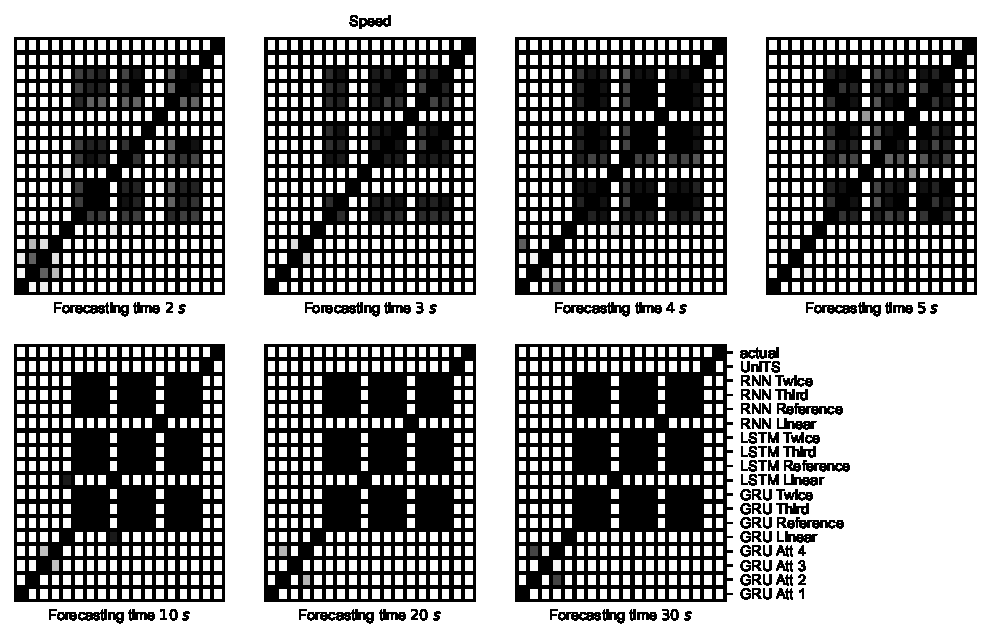
\includegraphics[width = 0.99 \linewidth]{var_speed.pdf}
	\caption{The $p$-values for the Wilcoxon signed-rank test on actual and predicted values across $k$-fold validation datasets for the speed in the $k$-fold testing datasets using different RNN models, and forecasting times. Darker colors in grayscale represent a higher $p$-value in a range from $0$ to $1$. The values on the secondary diagonal are all equal to $1$ and black because models equal themselves.}
	\label{fig:var_speed}
\end{figure}

The average RMSE, with standard deviation in brackets, across $k$-fold validation datasets for the speed estimated on the $k$-fold testing datasets by different RNN models, and forecasting times is listed in Table~\ref{tab:best_speed_RMSE}.

\begin{table}[!ht]
	\centering
	\resizebox{\linewidth}{!}{
		\begin{tabular}{|c|c|c|c|c|c|c|c|}
			\hline
			Model & $2$ $s$ & $3$ $s$ & $4$ $s$ & $5$ $s$ & $10$ $s$ & $20$ $s$ & $30$ $s$ \\ \hline
			\multirow{2}{*}{LSTM Linear} & $\mathbf{4.03}$ & $5.61$ & $6.87$ & $7.88$ & $10.37$ & $11.43$ & $11.9$ \\
			 & \textbf{(}$\mathbf{0.3}$\textbf{)} & ($0.45$) & ($0.53$) & ($0.59$) & ($0.71$) & ($0.75$) & ($0.76$) \\ \hline
			\multirow{2}{*}{UniTS} & $4.35$ & $\mathbf{5.25}$ & $\mathbf{6.02}$ & $\mathbf{6.69}$ & $\mathbf{8.86}$ & $\mathbf{10.55}$ & $\mathbf{11.26}$ \\
			 & ($0.3$) & \textbf{(}$\mathbf{0.37}$\textbf{)} & \textbf{(}$\mathbf{0.42}$\textbf{)} & \textbf{(}$\mathbf{0.47}$\textbf{)} & \textbf{(}$\mathbf{0.64}$\textbf{)} & \textbf{(}$\mathbf{0.77}$\textbf{)} & \textbf{(}$\mathbf{0.75}$\textbf{)} \\ \hline
		\end{tabular}
	}
	\caption{The average RMSE, with standard deviation in brackets, across $k$-fold validation datasets for the speed estimated on the $k$-fold testing datasets by different RNN models, and forecasting times.}
	\label{tab:best_speed_RMSE}
\end{table}

The LSTM Linear model achieved the lowest RMSE for speed, and a forecasting time of $2$ $s$ with an average value and standard deviation (in brackets) that equals $4.03$ $km/h$ ($0.3$ $km/h$).

The LSTM Linear model does not have a statistically significantly different RMSE than the GRU Linear, and RNN Linear models for speed using a forecasting time of $2$ $s$, with $p$-values equaling $2.099 \times 10^{-1}$, and $2.002 \times 10^{-1}$.

The UniTS model achieved the lowest RMSE for speed, and a forecasting time of $3$, $4$, $5$, $10$, $20$, and $30$ $s$ with average values and standard deviation (in brackets) that equal $5.25$ $km/h$ ($0.37$ $km/h$), $6.02$ $km/h$ ($0.42$ $km/h$), $6.69$ $km/h$ ($0.47$ $km/h$), $8.86$ $km/h$ ($0.64$ $km/h$), $10.55$ $km/h$ ($0.77$ $km/h$), and $11.26$ $km/h$ ($0.75$ $km/h$) respectively.

\subsection{Results for Trajectories Estimated Using $x$ and $y$ Offset}
%\label{subsec:no_abs_results}
%\vspace{10pt}

Figure~\ref{fig:best_RMSE_traj_val} contains the average RMSE across $k$-fold testing datasets using different trajectory estimation methods, validation datasets for all trajectories estimated in nested $k$-fold cross-validation by different trajectory estimation methods, RNN models, and forecasting times.

\begin{figure}[!ht]
	\centering
	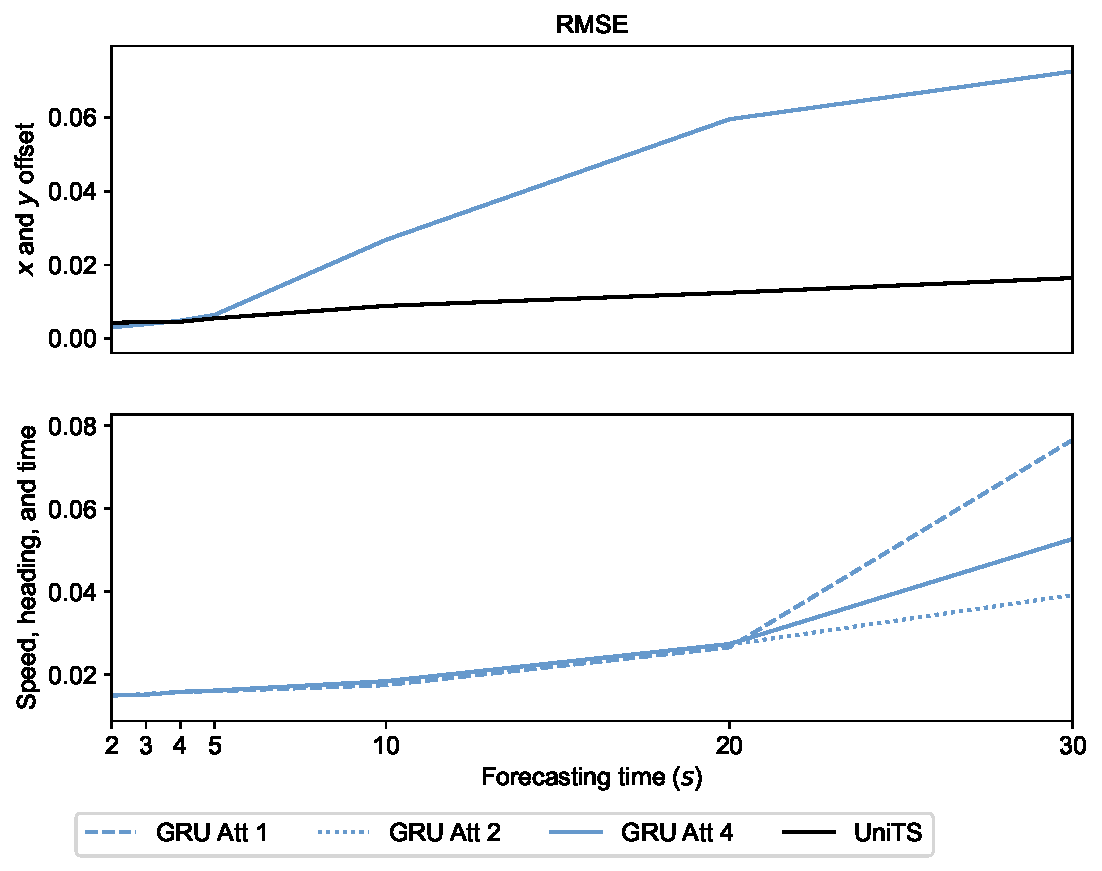
\includegraphics[width = 0.99 \linewidth]{best_RMSE_traj_val.pdf}
	\caption{The average RMSE across $k$-fold testing datasets using different trajectory estimation methods, validation datasets for all trajectories estimated in nested $k$-fold cross-validation by different trajectory estimation methods, RNN models, and forecasting times.}
	\label{fig:best_RMSE_traj_val}
\end{figure}

The average RMSE ($\times 10^{-3}$), with standard deviation in brackets, across $k$-fold validation datasets for the trajectories in the $k$-fold testing datasets estimated using $x$ and $y$ offset, different RNN models, and forecasting times is listed in Table~\ref{tab:best_no_abs_RMSE}.

\begin{table}[!ht]
	\centering
	\resizebox{\linewidth}{!}{
		\begin{tabular}{|c|c|c|c|c|c|c|c|}
			\hline
			Model & $2$ $s$ & $3$ $s$ & $4$ $s$ & $5$ $s$ & $10$ $s$ & $20$ $s$ & $30$ $s$ \\ \hline
			\multirow{2}{*}{GRU Att 4} & $\mathbf{3.05}$ & $\mathbf{3.86}$ & $4.86$ & $6.4$ & $26.8$ & $59.52$ & $72.49$ \\
			 & \textbf{(}$\mathbf{0.49}$\textbf{)} & \textbf{(}$\mathbf{0.51}$\textbf{)} & ($0.52$) & ($0.85$) & ($6.96$) & ($9.83$) & ($19.4$) \\ \hline
			\multirow{2}{*}{UniTS} & $4.26$ & $4.47$ & $\mathbf{4.54}$ & $\mathbf{5.47}$ & $\mathbf{8.86}$ & $\mathbf{12.43}$ & $\mathbf{16.41}$ \\
			 & ($3.51$) & ($2.91$) & \textbf{(}$\mathbf{0.66}$\textbf{)} & \textbf{(}$\mathbf{0.97}$\textbf{)} & \textbf{(}$\mathbf{1.37}$\textbf{)} & \textbf{(}$\mathbf{1.55}$\textbf{)} & \textbf{(}$\mathbf{2.47}$\textbf{)} \\ \hline
		\end{tabular}
	}
	\caption{The average RMSE ($\times 10^{-3}$), with standard deviation in brackets, across $k$-fold validation datasets for the trajectories in the $k$-fold testing datasets estimated using $x$ and $y$ offset, different RNN models, and forecasting times.}
	\label{tab:best_no_abs_RMSE}
\end{table}

The GRU Att 4 model achieved the lowest RMSE for trajectories estimated using $x$ and $y$ offset, and a forecasting time of $2$, and $3$ $s$ with average values and standard deviation (in brackets) that equal $3.05 \times 10^{-3}$ $\degree$ ($0.49 \times 10^{-3}$ $\degree$), and $3.86 \times 10^{-3}$ $\degree$ ($0.51 \times 10^{-3}$ $\degree$) respectively.

The UniTS model achieved the lowest RMSE for trajectories estimated using $x$ and $y$ offset, and a forecasting time of $4$, $5$, $10$, $20$, and $30$ $s$ with average values and standard deviation (in brackets) that equal $4.54 \times 10^{-3}$ $\degree$ ($0.66 \times 10^{-3}$ $\degree$), $5.47 \times 10^{-3}$ $\degree$ ($0.97 \times 10^{-3}$ $\degree$), $8.86 \times 10^{-3}$ $\degree$ ($1.37 \times 10^{-3}$ $\degree$), $12.43 \times 10^{-3}$ $\degree$ ($1.55 \times 10^{-3}$ $\degree$), and $16.41 \times 10^{-3}$ $\degree$ ($2.47 \times 10^{-3}$ $\degree$) respectively.

\subsection{Results for Trajectories Estimated Using Speed, Heading, and Time}
%\label{subsec:speed_actual_dir_results}
%\vspace{10pt}

The average RMSE ($\times 10^{-2}$), with standard deviation in brackets, across $k$-fold validation datasets for the trajectories in the $k$-fold testing datasets estimated using speed, heading, and time, different RNN models, and forecasting times is listed in Table~\ref{tab:best_speed_actual_dir_RMSE}.

\begin{table}[!ht]
	\centering
	\resizebox{\linewidth}{!}{
		\begin{tabular}{|c|c|c|c|c|c|c|c|}
			\hline
			Model & $2$ $s$ & $3$ $s$ & $4$ $s$ & $5$ $s$ & $10$ $s$ & $20$ $s$ & $30$ $s$ \\ \hline
			\multirow{2}{*}{GRU Att 1} & $1.501$ & $1.524$ & $1.587$ & $\mathbf{1.598}$ & $\mathbf{1.745}$ & $\mathbf{2.657}$ & $7.659$ \\
			 & ($0.163$) & ($0.154$) & ($0.163$) & \textbf{(}$\mathbf{0.135}$\textbf{)} & \textbf{(}$\mathbf{0.108}$\textbf{)} & \textbf{(}$\mathbf{0.17}$\textbf{)} & ($6.196$) \\ \hline
			\multirow{2}{*}{GRU Att 2} & $1.495$ & $1.536$ & $1.586$ & $1.616$ & $1.818$ & $2.72$ & $\mathbf{3.919}$ \\
			 & ($0.161$) & ($0.177$) & ($0.173$) & ($0.165$) & ($0.192$) & ($0.19$) & \textbf{(}$\mathbf{0.589}$\textbf{)} \\ \hline
			\multirow{2}{*}{GRU Att 4} & $\mathbf{1.494}$ & $\mathbf{1.514}$ & $\mathbf{1.581}$ & $1.616$ & $1.842$ & $2.737$ & $5.269$ \\
			 & \textbf{(}$\mathbf{0.152}$\textbf{)} & \textbf{(}$\mathbf{0.163}$\textbf{)} & \textbf{(}$\mathbf{0.173}$\textbf{)} & ($0.15$) & ($0.125$) & ($0.238$) & ($4.403$) \\ \hline
		\end{tabular}
	}
	\caption{The average RMSE ($\times 10^{-2}$), with standard deviation in brackets, across $k$-fold validation datasets for the trajectories in the $k$-fold testing datasets estimated using speed, heading, and time, different RNN models, and forecasting times.}
	\label{tab:best_speed_actual_dir_RMSE}
\end{table}

The GRU Att 1 model achieved the lowest RMSE for trajectories estimated using speed, heading, and time, and a forecasting time of $10$, $20$, and $5$ $s$ with average values and standard deviation (in brackets) that equal $17.45 \times 10^{-3}$ $\degree$ ($1.08 \times 10^{-3}$ $\degree$), $26.57 \times 10^{-3}$ $\degree$ ($1.7 \times 10^{-3}$ $\degree$), and $15.98 \times 10^{-3}$ $\degree$ ($1.35 \times 10^{-3}$ $\degree$) respectively.

The GRU Att 2 model achieved the lowest RMSE for trajectories estimated using speed, heading, and time, and a forecasting time of $30$ $s$ with an average value and standard deviation (in brackets) that equals $39.19 \times 10^{-3}$ $\degree$ ($5.89 \times 10^{-3}$ $\degree$).

The GRU Att 4 model achieved the lowest RMSE for trajectories estimated using speed, heading, and time, and a forecasting time of $2$, $3$, and $4$ $s$ with average values and standard deviation (in brackets) that equal $14.94 \times 10^{-3}$ $\degree$ ($1.52 \times 10^{-3}$ $\degree$), $15.14 \times 10^{-3}$ $\degree$ ($1.63 \times 10^{-3}$ $\degree$), and $15.81 \times 10^{-3}$ $\degree$ ($1.73 \times 10^{-3}$ $\degree$) respectively.

